\section{Codifica di sorgenti correlate}
\label{sec:correlated-sources-encoding}

Dal teorema di Shannon sulla codifica di sorgente
\cite{10.1002/j.1538-7305.1948.tb01338.x} è noto che per codificare una
sorgente \(X\), un tasso \(R > \entropy{X}\) è sufficiente. Consideriamo ora
due sorgenti correlate \((X,Y) \sim p(x, y)\). In questo caso, un tasso pari a
\(\entropy{X,Y}\) è sufficiente per codificarle congiuntamente. Supponiamo che
al ricevitore si desideri ricostruire \(X\) e \(Y\) separatamente. Si vede
facilmente che un tasso \(R = R_X + R_Y > \entropy{X} + \entropy{Y}\) è
sufficiente. Tuttavia, Slepian e Wolf \cite{1055037} hanno dimostrato che un
tasso totale pari a \(R = \entropy{X,Y}\) è sufficiente anche per codificare
separatamente le due sorgenti correlate.

Riportiamo nel seguito il teorema di Slepian-Wolf
\cite{10.1002/047174882X.ch15}. In Figura~\ref{fig:sw-configuration} è
illustrata la situazione considerata.

\begin{figure}[ht]
    \centering
    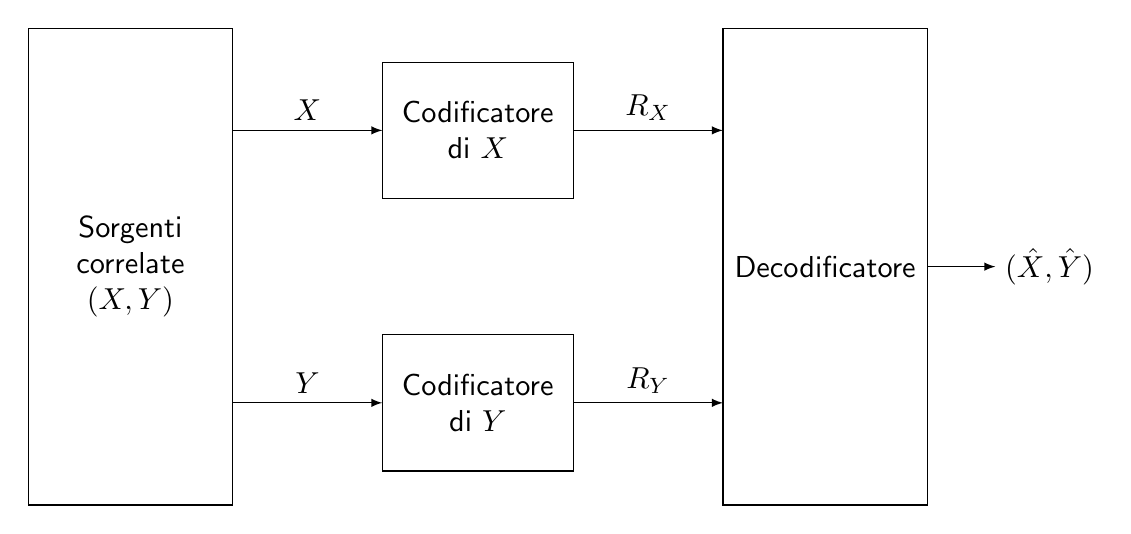
\begin{tikzpicture}[scale=0.865,>=latex]
    \tikzstyle{every node}=[font=\fontsize{11}{13}\sffamily]

    \draw (0,0) rectangle (3,7)
    node[midway,align=center]{Sorgenti \\ correlate \\ \((X,Y)\)};

    \draw[->] (3,5.5) -- (5.2,5.5)
    node[above,midway]{\(X\)};

    \draw[->] (3,1.5) -- (5.2,1.5)
    node[above,midway]{\(Y\)};

    \draw (5.2,4.5) rectangle (8,6.5)
    node[midway,align=center]{Codificatore \\ di \(X\)};

    \draw (5.2,0.5) rectangle (8,2.5)
    node[midway,align=center]{Codificatore \\ di \(Y\)};

    \draw[->] (8,5.5) -- (10.2,5.5)
    node[above,midway]{\(R_X\)};

    \draw[->] (8,1.5) -- (10.2,1.5)
    node[above,midway]{\(R_Y\)};

    \draw (10.2,0) rectangle (13.2,7)
    node[midway]{Decodificatore};

    \draw[->] (13.2,3.5) -- (14.2,3.5)
    node[right]{\((\hat{X},\hat{Y})\)};
\end{tikzpicture}

    \caption{Configurazione per la codifica di sorgente Slepian-Wolf.}
    \label{fig:sw-configuration}
\end{figure}

\begin{thm}[Slepian-Wolf \textnormal{\cite{10.1002/047174882X.ch15}}]
    \label{thm:sw}

    Sia \((X_1,Y_1),(X_2,Y_2),\dots\) una sequenza di variabili aleatorie
    indipendenti e identicamente distribuite, tali che la generica coppia
    \((X,Y) \sim p(x, y)\), con \(X\) e \(Y\) congiunte.\\
    Per il problema della codifica di sorgenti distribuite per la sorgente
    \((X,Y)\), la regione di tasso raggiungibile è data da
    \begin{alignat}{1}
        R_X &\ge \entropy{X \given Y}, \label{eq:SW1} \\
        R_Y &\ge \entropy{Y \given X}, \label{eq:SW2} \\
        R_X + R_Y &\ge \entropy{X,Y}. \label{eq:SWsum}
    \end{alignat}
\end{thm}

La Figura~\ref{fig:sw-rate-region} mostra la regione descritta dal
Teorema~\ref{thm:sw}.

\begin{figure}[ht]
    \centering
    \begin{tikzpicture}[>=latex]
    \draw[->] (0,0) -- (8,0)
    node[right]{\(R_X\)};

    \draw[->] (0,0) -- (0,6)
    node[above]{\(R_Y\)};

    \draw (1.8,3pt) -- (1.8,-3pt)
    node[anchor=north]{\(\entropy{X \given Y}\)};

    \draw (3.6,3pt) -- (3.6,-3pt)
    node[anchor=north]{\(\entropy{X}\)};

    \draw (7.2,3pt) -- (7.2,-3pt)
    node[anchor=north]{\(\entropy{X,Y}\)};

    \draw (3pt,2) -- (-3pt,2)
    node[anchor=east]{\(\entropy{Y \given X}\)};

    \draw (3pt,3) -- (-3pt,3)
    node[anchor=east]{\(\entropy{Y}\)};

    \draw (3pt,4) -- (-3pt,4)
    node[anchor=east]{\(\entropy{X,Y}\)};

    \draw[help lines] (7.2,0) -- (0,4);
    \draw[help lines] (1.8,0) -- (1.8,5.5);
    \draw[help lines] (3.6,0) -- (3.6,2);
    \draw[help lines] (0,2) -- (7,2);
    \draw[help lines] (0,3) -- (1.8,3);

    \draw (3.6,2) -- (7,2);
    \draw (3.6,2) -- (1.8,3);
    \draw (1.8,5.5) -- (1.8,3);

    \foreach \x in {2.64,2.74,...,6}
    \draw[xslant=0.5] (\x cm,2) -- (\x cm,2.22);

    \foreach \x in {0.2,0.3,...,2.2}
    \draw[rotate=-29.055] (\x cm,3.5) -- (\x cm,3.75);

    \foreach \y in {-0.2,-0.04,...,2.22}
    \draw[yslant=1.8] (1.8,\y cm) -- (1.925,\y cm);

    \draw (4,3.5) node{\(\set{R}\)};
\end{tikzpicture}

    \caption{Regione \(\set{R}\) di tasso raggiungibile con la codifica di
    sorgente Slepian-Wolf.}
    \label{fig:sw-rate-region}
\end{figure}
